
%% bare_conf.tex
%% V1.4b
%% 2015/08/26
%% by Michael Shell
%% See:
%% http://www.michaelshell.org/
%% for current contact information.
%%
%% This is a skeleton file demonstrating the use of IEEEtran.cls
%% (requires IEEEtran.cls version 1.8b or later) with an IEEE
%% conference paper.
%%
%% Support sites:
%% http://www.michaelshell.org/tex/ieeetran/
%% http://www.ctan.org/pkg/ieeetran
%% and
%% http://www.ieee.org/

%%*************************************************************************
%% Legal Notice:
%% This code is offered as-is without any warranty either expressed or
%% implied; without even the implied warranty of MERCHANTABILITY or
%% FITNESS FOR A PARTICULAR PURPOSE! 
%% User assumes all risk.
%% In no event shall the IEEE or any contributor to this code be liable for
%% any damages or losses, including, but not limited to, incidental,
%% consequential, or any other damages, resulting from the use or misuse
%% of any information contained here.
%%
%% All comments are the opinions of their respective authors and are not
%% necessarily endorsed by the IEEE.
%%
%% This work is distributed under the LaTeX Project Public License (LPPL)
%% ( http://www.latex-project.org/ ) version 1.3, and may be freely used,
%% distributed and modified. A copy of the LPPL, version 1.3, is included
%% in the base LaTeX documentation of all distributions of LaTeX released
%% 2003/12/01 or later.
%% Retain all contribution notices and credits.
%% ** Modified files should be clearly indicated as such, including  **
%% ** renaming them and changing author support contact information. **
%%*************************************************************************


% *** Authors should verify (and, if needed, correct) their LaTeX system  ***
% *** with the testflow diagnostic prior to trusting their LaTeX platform ***
% *** with production work. The IEEE's font choices and paper sizes can   ***
% *** trigger bugs that do not appear when using other class files.       ***                          ***
% The testflow support page is at:
% http://www.michaelshell.org/tex/testflow/



\documentclass[conference]{IEEEtran}
% Some Computer Society conferences also require the compsoc mode option,
% but others use the standard conference format.
%
% If IEEEtran.cls has not been installed into the LaTeX system files,
% manually specify the path to it like:
% \documentclass[conference]{../sty/IEEEtran}





% Some very useful LaTeX packages include:
% (uncomment the ones you want to load)


% *** MISC UTILITY PACKAGES ***
%
%\usepackage{ifpdf}
% Heiko Oberdiek's ifpdf.sty is very useful if you need conditional
% compilation based on whether the output is pdf or dvi.
% usage:
% \ifpdf
%   % pdf code
% \else
%   % dvi code
% \fi
% The latest version of ifpdf.sty can be obtained from:
% http://www.ctan.org/pkg/ifpdf
% Also, note that IEEEtran.cls V1.7 and later provides a builtin
% \ifCLASSINFOpdf conditional that works the same way.
% When switching from latex to pdflatex and vice-versa, the compiler may
% have to be run twice to clear warning/error messages.






% *** CITATION PACKAGES ***
%
%\usepackage{cite}
% cite.sty was written by Donald Arseneau
% V1.6 and later of IEEEtran pre-defines the format of the cite.sty package
% \cite{} output to follow that of the IEEE. Loading the cite package will
% result in citation numbers being automatically sorted and properly
% "compressed/ranged". e.g., [1], [9], [2], [7], [5], [6] without using
% cite.sty will become [1], [2], [5]--[7], [9] using cite.sty. cite.sty's
% \cite will automatically add leading space, if needed. Use cite.sty's
% noadjust option (cite.sty V3.8 and later) if you want to turn this off
% such as if a citation ever needs to be enclosed in parenthesis.
% cite.sty is already installed on most LaTeX systems. Be sure and use
% version 5.0 (2009-03-20) and later if using hyperref.sty.
% The latest version can be obtained at:
% http://www.ctan.org/pkg/cite
% The documentation is contained in the cite.sty file itself.






% *** GRAPHICS RELATED PACKAGES ***
%
\ifCLASSINFOpdf
   \usepackage[pdftex]{graphicx}
  % declare the path(s) where your graphic files are
   \graphicspath{{./Abbildungen/}}
  % and their extensions so you won't have to specify these with
  % every instance of \includegraphics
   \DeclareGraphicsExtensions{.pdf}
\else
  % or other class option (dvipsone, dvipdf, if not using dvips). graphicx
  % will default to the driver specified in the system graphics.cfg if no
  % driver is specified.
  % \usepackage[dvips]{graphicx}
  % declare the path(s) where your graphic files are
  % \graphicspath{{../eps/}}
  % and their extensions so you won't have to specify these with
  % every instance of \includegraphics
  % \DeclareGraphicsExtensions{.eps}
\fi
% graphicx was written by David Carlisle and Sebastian Rahtz. It is
% required if you want graphics, photos, etc. graphicx.sty is already
% installed on most LaTeX systems. The latest version and documentation
% can be obtained at: 
% http://www.ctan.org/pkg/graphicx
% Another good source of documentation is "Using Imported Graphics in
% LaTeX2e" by Keith Reckdahl which can be found at:
% http://www.ctan.org/pkg/epslatex
%
% latex, and pdflatex in dvi mode, support graphics in encapsulated
% postscript (.eps) format. pdflatex in pdf mode supports graphics
% in .pdf, .jpeg, .png and .mps (metapost) formats. Users should ensure
% that all non-photo figures use a vector format (.eps, .pdf, .mps) and
% not a bitmapped formats (.jpeg, .png). The IEEE frowns on bitmapped formats
% which can result in "jaggedy"/blurry rendering of lines and letters as
% well as large increases in file sizes.
%
% You can find documentation about the pdfTeX application at:
% http://www.tug.org/applications/pdftex





% *** MATH PACKAGES ***
%
\usepackage{amsmath}
% A popular package from the American Mathematical Society that provides
% many useful and powerful commands for dealing with mathematics.
%
% Note that the amsmath package sets \interdisplaylinepenalty to 10000
% thus preventing page breaks from occurring within multiline equations. Use:
%\interdisplaylinepenalty=2500
% after loading amsmath to restore such page breaks as IEEEtran.cls normally
% does. amsmath.sty is already installed on most LaTeX systems. The latest
% version and documentation can be obtained at:
% http://www.ctan.org/pkg/amsmath

\usepackage{amssymb}



% *** SPECIALIZED LIST PACKAGES ***
%
%\usepackage{algorithmic}
% algorithmic.sty was written by Peter Williams and Rogerio Brito.
% This package provides an algorithmic environment fo describing algorithms.
% You can use the algorithmic environment in-text or within a figure
% environment to provide for a floating algorithm. Do NOT use the algorithm
% floating environment provided by algorithm.sty (by the same authors) or
% algorithm2e.sty (by Christophe Fiorio) as the IEEE does not use dedicated
% algorithm float types and packages that provide these will not provide
% correct IEEE style captions. The latest version and documentation of
% algorithmic.sty can be obtained at:
% http://www.ctan.org/pkg/algorithms
% Also of interest may be the (relatively newer and more customizable)
% algorithmicx.sty package by Szasz Janos:
% http://www.ctan.org/pkg/algorithmicx




% *** ALIGNMENT PACKAGES ***
%
%\usepackage{array}
% Frank Mittelbach's and David Carlisle's array.sty patches and improves
% the standard LaTeX2e array and tabular environments to provide better
% appearance and additional user controls. As the default LaTeX2e table
% generation code is lacking to the point of almost being broken with
% respect to the quality of the end results, all users are strongly
% advised to use an enhanced (at the very least that provided by array.sty)
% set of table tools. array.sty is already installed on most systems. The
% latest version and documentation can be obtained at:
% http://www.ctan.org/pkg/array


% IEEEtran contains the IEEEeqnarray family of commands that can be used to
% generate multiline equations as well as matrices, tables, etc., of high
% quality.




% *** SUBFIGURE PACKAGES ***
%\ifCLASSOPTIONcompsoc
%  \usepackage[caption=false,font=normalsize,labelfont=sf,textfont=sf]{subfig}
%\else
%  \usepackage[caption=false,font=footnotesize]{subfig}
%\fi
% subfig.sty, written by Steven Douglas Cochran, is the modern replacement
% for subfigure.sty, the latter of which is no longer maintained and is
% incompatible with some LaTeX packages including fixltx2e. However,
% subfig.sty requires and automatically loads Axel Sommerfeldt's caption.sty
% which will override IEEEtran.cls' handling of captions and this will result
% in non-IEEE style figure/table captions. To prevent this problem, be sure
% and invoke subfig.sty's "caption=false" package option (available since
% subfig.sty version 1.3, 2005/06/28) as this is will preserve IEEEtran.cls
% handling of captions.
% Note that the Computer Society format requires a larger sans serif font
% than the serif footnote size font used in traditional IEEE formatting
% and thus the need to invoke different subfig.sty package options depending
% on whether compsoc mode has been enabled.
%
% The latest version and documentation of subfig.sty can be obtained at:
% http://www.ctan.org/pkg/subfig




% *** FLOAT PACKAGES ***
%
%\usepackage{fixltx2e}
% fixltx2e, the successor to the earlier fix2col.sty, was written by
% Frank Mittelbach and David Carlisle. This package corrects a few problems
% in the LaTeX2e kernel, the most notable of which is that in current
% LaTeX2e releases, the ordering of single and double column floats is not
% guaranteed to be preserved. Thus, an unpatched LaTeX2e can allow a
% single column figure to be placed prior to an earlier double column
% figure.
% Be aware that LaTeX2e kernels dated 2015 and later have fixltx2e.sty's
% corrections already built into the system in which case a warning will
% be issued if an attempt is made to load fixltx2e.sty as it is no longer
% needed.
% The latest version and documentation can be found at:
% http://www.ctan.org/pkg/fixltx2e


%\usepackage{stfloats}
% stfloats.sty was written by Sigitas Tolusis. This package gives LaTeX2e
% the ability to do double column floats at the bottom of the page as well
% as the top. (e.g., "\begin{figure*}[!b]" is not normally possible in
% LaTeX2e). It also provides a command:
%\fnbelowfloat
% to enable the placement of footnotes below bottom floats (the standard
% LaTeX2e kernel puts them above bottom floats). This is an invasive package
% which rewrites many portions of the LaTeX2e float routines. It may not work
% with other packages that modify the LaTeX2e float routines. The latest
% version and documentation can be obtained at:
% http://www.ctan.org/pkg/stfloats
% Do not use the stfloats baselinefloat ability as the IEEE does not allow
% \baselineskip to stretch. Authors submitting work to the IEEE should note
% that the IEEE rarely uses double column equations and that authors should try
% to avoid such use. Do not be tempted to use the cuted.sty or midfloat.sty
% packages (also by Sigitas Tolusis) as the IEEE does not format its papers in
% such ways.
% Do not attempt to use stfloats with fixltx2e as they are incompatible.
% Instead, use Morten Hogholm'a dblfloatfix which combines the features
% of both fixltx2e and stfloats:
%
% \usepackage{dblfloatfix}
% The latest version can be found at:
% http://www.ctan.org/pkg/dblfloatfix




% *** PDF, URL AND HYPERLINK PACKAGES ***
%
%\usepackage{url}
% url.sty was written by Donald Arseneau. It provides better support for
% handling and breaking URLs. url.sty is already installed on most LaTeX
% systems. The latest version and documentation can be obtained at:
% http://www.ctan.org/pkg/url
% Basically, \url{my_url_here}.




% *** Do not adjust lengths that control margins, column widths, etc. ***
% *** Do not use packages that alter fonts (such as pslatex).         ***
% There should be no need to do such things with IEEEtran.cls V1.6 and later.
% (Unless specifically asked to do so by the journal or conference you plan
% to submit to, of course. )


% correct bad hyphenation here
\hyphenation{op-tical net-works semi-conduc-tor}

%------------------------Thilo Package Area-----------------------------
%Package for writing german letters
\usepackage[utf8]{inputenc}

%-----------------------------------------------------------------------
\begin{document}
%
% paper title
% Titles are generally capitalized except for words such as a, an, and, as,
% at, but, by, for, in, nor, of, on, or, the, to and up, which are usually
% not capitalized unless they are the first or last word of the title.
% Linebreaks \\ can be used within to get better formatting as desired.
% Do not put math or special symbols in the title.
\title{(Deep) Reinforcement Learning - \\ Policy Gradient}


% author names and affiliations
% use a multiple column layout for up to three different
% affiliations
\author{\IEEEauthorblockN{Thilo Stegemann}
\IEEEauthorblockA{Hochschule für Technik und Wirtschaft\\Master Student der Angewandten Informatik\\
12459 Berlin, Wilhelminenhofstraße 75A\\
Email: t.stegemann@gmx.de}}

% conference papers do not typically use \thanks and this command
% is locked out in conference mode. If really needed, such as for
% the acknowledgment of grants, issue a \IEEEoverridecommandlockouts
% after \documentclass

% for over three affiliations, or if they all won't fit within the width
% of the page, use this alternative format:
% 
%\author{\IEEEauthorblockN{Michael Shell\IEEEauthorrefmark{1},
%Homer Simpson\IEEEauthorrefmark{2},
%James Kirk\IEEEauthorrefmark{3}, 
%Montgomery Scott\IEEEauthorrefmark{3} and
%Eldon Tyrell\IEEEauthorrefmark{4}}
%\IEEEauthorblockA{\IEEEauthorrefmark{1}School of Electrical and Computer Engineering\\
%Georgia Institute of Technology,
%Atlanta, Georgia 30332--0250\\ Email: see http://www.michaelshell.org/contact.html}
%\IEEEauthorblockA{\IEEEauthorrefmark{2}Twentieth Century Fox, Springfield, USA\\
%Email: homer@thesimpsons.com}
%\IEEEauthorblockA{\IEEEauthorrefmark{3}Starfleet Academy, San Francisco, California 96678-2391\\
%Telephone: (800) 555--1212, Fax: (888) 555--1212}
%\IEEEauthorblockA{\IEEEauthorrefmark{4}Tyrell Inc., 123 Replicant Street, Los Angeles, California 90210--4321}}




% use for special paper notices
%\IEEEspecialpapernotice{(Invited Paper)}




% make the title area
\maketitle

% As a general rule, do not put math, special symbols or citations
% in the abstract
\begin{abstract}
The abstract goes here.
\end{abstract}

% no keywords




% For peer review papers, you can put extra information on the cover
% page as needed:
% \ifCLASSOPTIONpeerreview
% \begin{center} \bfseries EDICS Category: 3-BBND \end{center}
% \fi
%
% For peerreview papers, this IEEEtran command inserts a page break and
% creates the second title. It will be ignored for other modes.
\IEEEpeerreviewmaketitle



\section{Einführung}
% no \IEEEPARstart
This demo file is intended to serve as a ``starter file''
for IEEE conference papers produced under \LaTeX\ using
IEEEtran.cls version 1.8b and later.
% You must have at least 2 lines in the paragraph with the drop letter
% (should never be an issue)
I wish you the best of success.

\hfill mds
 
\hfill August 26, 2015

% An example of a floating figure using the graphicx package.
% Note that \label must occur AFTER (or within) \caption.
% For figures, \caption should occur after the \includegraphics.
% Note that IEEEtran v1.7 and later has special internal code that
% is designed to preserve the operation of \label within \caption
% even when the captionsoff option is in effect. However, because
% of issues like this, it may be the safest practice to put all your
% \label just after \caption rather than within \caption{}.
%
% Reminder: the "draftcls" or "draftclsnofoot", not "draft", class
% option should be used if it is desired that the figures are to be
% displayed while in draft mode.
%
%\begin{figure}[!t]
%\centering
%\includegraphics[width=2.5in]{myfigure}
% where an .eps filename suffix will be assumed under latex, 
% and a .pdf suffix will be assumed for pdflatex; or what has been declared
% via \DeclareGraphicsExtensions.
%\caption{Simulation results for the network.}
%\label{fig_sim}
%\end{figure}

% Note that the IEEE typically puts floats only at the top, even when this
% results in a large percentage of a column being occupied by floats.


% An example of a double column floating figure using two subfigures.
% (The subfig.sty package must be loaded for this to work.)
% The subfigure \label commands are set within each subfloat command,
% and the \label for the overall figure must come after \caption.
% \hfil is used as a separator to get equal spacing.
% Watch out that the combined width of all the subfigures on a 
% line do not exceed the text width or a line break will occur.
%
%\begin{figure*}[!t]
%\centering
%\subfloat[Case I]{\includegraphics[width=2.5in]{box}%
%\label{fig_first_case}}
%\hfil
%\subfloat[Case II]{\includegraphics[width=2.5in]{box}%
%\label{fig_second_case}}
%\caption{Simulation results for the network.}
%\label{fig_sim}
%\end{figure*}
%
% Note that often IEEE papers with subfigures do not employ subfigure
% captions (using the optional argument to \subfloat[]), but instead will
% reference/describe all of them (a), (b), etc., within the main caption.
% Be aware that for subfig.sty to generate the (a), (b), etc., subfigure
% labels, the optional argument to \subfloat must be present. If a
% subcaption is not desired, just leave its contents blank,
% e.g., \subfloat[].


% An example of a floating table. Note that, for IEEE style tables, the
% \caption command should come BEFORE the table and, given that table
% captions serve much like titles, are usually capitalized except for words
% such as a, an, and, as, at, but, by, for, in, nor, of, on, or, the, to
% and up, which are usually not capitalized unless they are the first or
% last word of the caption. Table text will default to \footnotesize as
% the IEEE normally uses this smaller font for tables.
% The \label must come after \caption as always.
%
%\begin{table}[!t]
%% increase table row spacing, adjust to taste
%\renewcommand{\arraystretch}{1.3}
% if using array.sty, it might be a good idea to tweak the value of
% \extrarowheight as needed to properly center the text within the cells
%\caption{An Example of a Table}
%\label{table_example}
%\centering
%% Some packages, such as MDW tools, offer better commands for making tables
%% than the plain LaTeX2e tabular which is used here.
%\begin{tabular}{|c||c|}
%\hline
%One & Two\\
%\hline
%Three & Four\\
%\hline
%\end{tabular}
%\end{table}


% Note that the IEEE does not put floats in the very first column
% - or typically anywhere on the first page for that matter. Also,
% in-text middle ("here") positioning is typically not used, but it
% is allowed and encouraged for Computer Society conferences (but
% not Computer Society journals). Most IEEE journals/conferences use
% top floats exclusively. 
% Note that, LaTeX2e, unlike IEEE journals/conferences, places
% footnotes above bottom floats. This can be corrected via the
% \fnbelowfloat command of the stfloats package.

% conference papers do not normally have an appendix


\section{Reinforcement Learning (RL)}
Sutton und Barto \cite{sutton_barto_12} definieren ein Standard Reinforcement Learning Framework, in diesem interagiert ein Agent mit einer Umgebung. Dieses standart RL-Framework wird nachfolgend ausführlich beschrieben, denn es ist eine elementare Grundlage für das Verständnis des Policy Gradient Verfahrens. Der Agent lernt, in einer ihm unbekannten Umgebung, durch Versuch und Irrtum eine Strategie $\pi$ (eng. Policy). Der Agent kann in einer bestimmten Umgebung bestimmte Aktionen $a$ ausführen. Ist die Menge der Aktionen begrenzt, dann ist es ein diskreter Aktionsraum $A$. Eine unbegrenzte Menge von Aktionen bezeichnet einen kontinuierlichen Aktionsraum. Die Umgebung bestimmt die Aktionsmenge und der Agent entscheidet welche Aktion aus dieser Menge ausgewählt wird. Eine Aktion kann eine Positionsangabe, eine Richtung oder etwas viel komplexeres sein. Sutton und Barto \cite{sutton_barto_12} definieren die Umgebung als einen Markov Entscheidungsprozess (eng. \textbf{M}arkov \textbf{D}ecision \textbf{P}rocess). Der Agent interagiert demnach mit einem MDP und erhält von diesem einen Zustand und eine Belohnung. Der MDP erhält vom Agenten eine ausgewählte Aktion. 

\subsection{Markov Decision Process}
Ein MDP ist ein sequentielles Entscheidungsproblem. Eine Sequenz $... S_t, A_t, R_{t+1}, S_{t+1}, A_{t+1}, R_{t+2}, S_{t+2} ...$ beschreibt die Interaktion des Agenten mit dem MDP. Ein Zustand ist eine Darstellung der Umwelt zu einem Zeitpunkt t. Die Zustände bestimmten, welche Aktionen ausgeführt werden können d.h. es existiert eine Funktion $A(S_t)$. Ergebnis dieser Funktion ist eine zulässige Menge von Aktionen $A_t$ in einem Zustand $S_t$. Der Agent erhält eine direkte Belohnung $R_{t+1}$ für das Ausführen einer Aktion $A_t$ in einem Zustand $S_t$. Ein Beispiel: Es existiert ein Tic Tac Toe Spiel mit 9 Spielfeldern. Das Tic Tac Toe Spiel ist die Umgebung. Eine Darstellungsmöglichkeit des Spielfelds ist z.B. eine 3x3 Matrix. Jedes Element der Matrix wird mit einem Leerzeichen (' ') initialisiert. Der Startzustand $s_0 \in S$ ist eine 3x3 Matrix, indem jedes Element der Matrix ein Leerzeichen ist. Ein Spieler kann Kreuze ('X') in die Matrix einfügen und der andere Spieler Kreise ('O'). Der gesamte Zustandsraum $S$ eines Tic Tac Toe Spiels, kann abgebildet werden. Die leeren Matrixelemente bestimmten die Positionen auf die Spielsteine gesetzt werden können. $A(s_0) = \{ (0,0), (0,1), ... , (2,1), (2,2)\}$ und die Policy $\pi(s_0) = a_0$ legt fest, welche Aktion $a_0$ im Startzustand $s_0$ ausgeführt werden soll ($a_0 \in A(s_0)$). Eine direkte Belohnung $R_{t+1}(s_t,a_t)$ ungleich $0$ erhält der Agent für dieses Beispiel erst, wenn ein Spieler gewinnt oder verliert. Ein weiteres Beispiel: Ein Modellhubschrauber soll eigenständig lernen zu fliegen ohne abzustürzen und bestimmte Manöver auszuführen. In diesem Beispiel ist die Steuerung des Modellhubschraubers die zu lernende Strategie des RL Algorithmus. Eigenschaften der Umwelt sind unter anderem: Luftdruck, Position und Geschwindigkeit des Hubschraubers, Windgeschwindigkeit, Treibstoff. Die Modellierung der Zustände in diesem zweiten Beispiel ist ungleich komplexer verglichen mit dem ersten Beispiel. Zustände und Aktionen können sehr komplexe Objekte sein, dahingegen ist die Belohnung ein numerischer Wert und kein komplexes Objekt.

Die numerische Belohnung ist eine Bewertung der Aktion des Agenten. Der Agent versucht diese numerische Belohnung, über die Zeit, zu maximieren. Der Agent kann eine Belohnung von $+10$ erhalten (Hubschrauber um 360 Grad gedreht), wenn er in einem Zustand $s$ eine Aktion $a$ mit $s\in S$ und $a\in A$ ausführt. Der Agent kann auch eine negative numerische Belohnung von z.B. $-23$ erhalten (Hubschrauber abgestürzt). Der genaue Wert der Belohnung wird von der Umgebung definiert und der Agent kann diesen Wert nicht direkt beeinflussen oder verändern. Allein die Entscheidungen d.h. die Aktionsauswahl des Agenten entscheidet über die erhaltene Belohnung r. Die Umgebung definiert eine Belohnungsfunktion $R_s^a = E\{ r_{t+1} | s_t = s, a_t = a \}$. Diese Funktion ist eine Abbildung von Zustand-Aktionspaaren auf erwartete Belohnungen.

In einer realen Umgebung kann es passieren, dass der Agent selbst (z.B. ein einfacher Laufroboter oder ein Hubschrauber) eine Signalstörung empfängt oder eine Fehlfunktion seiner mechanischen Steuereinheiten hat. Die Umgebungsgegebenheiten können sich ebenfalls verschieben oder verändern (z.B. wechselnde Windrichtungen, Windstärken-Schwankungen, andere autonom agierende Agenten). Man bezeichnet diese Möglichkeiten als die Dynamiken der Umgebung. Abgebildet werden diese Dynamiken mittels Wahrscheinlichkeiten. Die Zustandsübergangswahrscheinlichkeit das ein Agent in Zustand $s_t$ mit der Aktion $a_t$ in den Zustand $s'_t$ übergeht ist definiert durch die Wahrscheinlichkeit $P^a_{ss'} = Pr \{ s_{t+1} = s' | s_t = s, a_t = a \}.$ Die Umgebungsdynamik beeinflusst auch die Policy $\pi$ und die Belohnungsfunktion $R^a_s$.

\begin{figure}[!t]
\centering
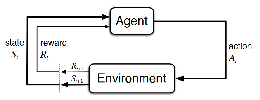
\includegraphics[width=2.5in]{agent_environment}
\caption{Die Interaktion zwischen Agent und Umgebung nach \cite{sutton_barto_12}.}
\label{agent_environment}
\end{figure}

\begin{figure}[!t]
\centering
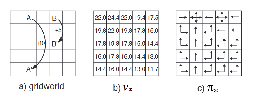
\includegraphics[width=3.5in]{gridworld_example}
\caption{Optimale Lösungen des Rasterwelt Beispiels nach \cite{sutton_barto_12}.}
\label{gridworld_example}
\end{figure}

\subsection{Die Strategie (Policy $\pi$)}
Die Policy ist eine Prozedur, welche die Entscheidungsfindung des Agenten festlegt. Eine Policy $\pi$ definiert das Verhalten des Agenten als Funktion von Zuständen $s$, mit $s \in S$ und $S$ ist der gesamte Zustandsraum. Eine stochastische angenäherte Policy wird als $\pi(s,a,\theta) = Pr \{ a_t = a | s_t = s, \theta \}$ geschrieben. 


Maximierung der Summe der erwarteten Belohnungen entspricht der Findung einer optimalen Strategie. \\

\paragraph*{Policy-Based Reinforcement Learning} 

$\pi$ is life!


\subsection{Die Bewertungsfunktion (Value Function)}
Bewertet wie gut jeder Zustand und/oder jede Aktion ist. \\

\paragraph*{Value-Based Reinforcement Learning} \mbox{}\\



\section{Policy Gradient Theorem}
Der Agent soll die Policy $\pi_\theta(s)$ mittels Erfahrung und daraus resultierender Belohnung und Bestrafung optimieren. Die folgenden zwei Optimierungsverfahren sind daher von besonderer Wichtigkeit, dass Gradienten Abstiegsverfahren (eng. Gradient Decent) und das Gradienten Anstiegsverfahren (eng. Gradient Ascent). Bei der univariaten und multivariaten Regression wird das Gradienten Abstiegsverfahren verwendet, um eine Kostenfunktion zu minimieren. Diese Kostenfunktion berechnet die Qualität einer Hypothese (z.B. mittels dem Fehler der kleinsten Quadrate eng. least-squared-errors). Bei Problemen des Reinforcement Learnings versucht der Agent eine möglichst optimale Strategie zu erlernen, daher versucht der Algorithmus des Agenten die abgeschwächten kumulierten Belohnungen über der Zeit zu maximieren mittels des Gradienten Anstiegsverfahrens. Um eine optimale Strategie zu entwickeln benötigt der Algorithmus folgende Elemente: Eine Zielfunktion, die die Qualität einer Policy $\pi$ bewertet, ein Verfahren welches die Zielfunktion maximiert und eine geeignete Darstellung der Policy $\pi$.

\subsection{Gradientenbasierte lokale Optimierung}
Eine Methode die Funktion $\pi_\theta(s)$ zu optimieren, ist das Gradienten Verfahren. Definition eines Gradienten nach G. Hoever \cite[vgl. S. 213]{hoever_14}: In einem Gradienten werden die verschiedenen partiellen Ableitungen einer Funktion $f(x)$ zusammengefasst. Zu einer Funktion $f : \mathbb{R}^n \rightarrow \mathbb{R}$ heißt (falls die partiellen Ableitungen existieren)

\begin{equation*}
\nabla f(x) := grad \: f(x) := \begin{pmatrix}
\frac{\partial f}{\partial x_1}(x), \hdots, \frac{\partial f}{\partial x_n}(x)
\end{pmatrix}
\end{equation*}

Gradient von $f$ im Punkt $x$. ($\nabla f$ wird "nabla $f$" gelesen.) Der Gradient einer Funktion weist in die Richtung des Steilsten Anstiegs. Senkrecht zum Gradienten ändert sich der Funktionswert nicht. G.Hoever \cite[vgl. S. 214]{hoever_14} liefert ebenfalls eine Erklärung des Gradientenverfahrens: Sucht man ausgehend von einem Startpunkt $x^{(0)}$ eine Maximalstelle (Gradient Ascent), so geht man ein Stück in die Richtung des Gradienten, also
\begin{equation*}
x^{(1)} = x^{(0)} + \alpha_0 \cdot \nabla \: f(x^{(0)}),
\end{equation*}
\begin{equation*}
x^{(2)} = x^{(1)} + \alpha_1 \cdot \nabla \: f(x^{(1)}),
\end{equation*}
allgemein:
\begin{equation*}
x^{(i+1)} = x^{(i)} + \alpha_i \cdot \nabla \: f(x^{(i)}).
\end{equation*}

Dabei beschreibt $\alpha_i$ die Schrittweite. Die genaue Wahl dieser Schrittweite ist oft nicht ganz einfach, wird an dieser Stelle jedoch nicht näher erläutert. Sucht man eine Minimalstelle (Gradient Descent), so setzt man entsprechend 

\begin{equation*}
x^{(i+1)} = x^{(i)} - \alpha_i \cdot \nabla \: f(x^{(i)}).
\end{equation*}

\subsection{Zielfunktion}
Die Qualität (Performance) einer Policy berechnet die Zielfunktion (eng. objective function oder criterion) $\rho(\pi)$. R. S. Sutton \cite{sutton_99} unterscheidet zwei verschiedene Formulierungen der Zielfunktion $\rho(\pi)$: 

\begin{equation*}
\begin{aligned}
\rho_{avR}(\pi) & = \lim\limits_{n \rightarrow \infty}{\frac{1}{n} E\{r_1 + r_2 + ... + r_n | \pi\}} \\
& = \sum_s d^\pi (s) \sum_a \pi(s,a) R^a_s,
\end{aligned}
\end{equation*}

ist die durchschnittliche Belohnung, diese bewertet die Strategie bezüglich der zu erwartenden Langzeitbelohnung pro Schritt. Eine Langzeitbelohnung (eng. long-term reward) ist die Aufsummierung der Belohnungen für eine Entscheidungssequenz. Der Term $d^\pi(s) = \lim\limits_{t \rightarrow \infty} Pr\{s_t = s|s_0,\pi\}$ beschreibt die stationäre Verteilung der Zustände unter $\pi$, d.h. $d^\pi(s)$ gibt an, wie hoch die Wahrscheinlichkeit dafür ist, jeden Zustand $s_t$ zu erreichen, bedingt durch die Policy $\pi$ und unabhängig vom Startzustand $s_0$, wenn $t$ gegen unendlich strebt. Sprachliche Formulierung der Funktion $\rho_{avR}(\pi)$: Es existiert eine Wahrscheinlichkeit, dass sich der Agent in Zustand $s$ befindet und es existiert eine Wahrscheinlichkeit, dass der Agent eine Aktion $a$ auswählt ($a$ abhängig von $\pi$). Berechnet wird die durchschnittliche Belohnung pro Zeitschritt, wobei die Belohnung $R^a_s$ von den beiden vorher erwähnten Wahrscheinlichkeiten $s$ und $a$ abhängt. Der Wert eines Zustands-Aktionspaares, unter Berücksichtigung einer Policy $\pi$, ist für die Zielfunktion der durchschnittlichen Belohnung $\rho_{avR}(\pi)$ wie folgt definiert:

\begin{equation*}
Q^\pi(s,a) = \sum^\infty_{t=1} E\{r_t - \rho_{avR}(\pi)|s_0 = s, a_0 = a, \pi\},
\end{equation*}

mit $\forall s \in S, a \in A$. Die Funktion berechnet die Summe der Differenzen zwischen einer sofortigen Belohnung ($r_t$) in jedem Zeitschritt $t$ und der Zielfunktion $\rho_{avR}(\pi)$, also der durchschnittlichen Belohnung pro Zeitschritt, für ein Zustands-Aktionspaar unter Verwendung einer Policy $\pi$. R. S. Sutton notiert die Zielfunktion $\rho_{avR}(\pi)$ als $\rho(\pi)$, in dieser Arbeit wird für die durchschnittliche erwartete Belohnung pro Zeitschritt die Notation $\rho_{avR}(\pi)$ verwendet (für \textbf{av}erage \textbf{R}eward ähnlich D. Silver \cite{silver_15}). Die zweite Formulierung der Zielfunktion $\rho(\pi)$ berücksichtigt einen genau festgelegten Startzustand $s_0$ und ausschließlich von diesem Startzustand ausgehende Langzeitbelohnungen:

\begin{equation*}
\rho_{s_0}(\pi) = E\{\sum^\infty_{t=1} \gamma^{t-1} r_t | s_0,\pi \}
\end{equation*}
und
\begin{equation*}
Q^\pi (s,a) = E \{\sum^\infty_{k=1} \gamma^{k-1} r_{t+k} | s_t = s, a_t = a, \pi\}.
\end{equation*}

Dabei ist $\gamma \in [0,1]$ ein Abschwächungsfaktor ($\gamma = 1$ ist nur in endlichen abzählbaren Sequenzen einzusetzen). Die stationäre Verteilung der Zustände $d^\pi (s)$ ist bei der Startzustandsformulierung eine abgeschwächte Gewichtung der vorgefundenen Zustände angefangen in Zustand $s_0$ und unter Berücksichtigung der Policy $\pi$: $d^\pi (s) = \sum^\infty_{t=0} \gamma^t Pr \{s_t = s | s_0, \pi\}$.
 
\section{Policy Gradient}

\begin{equation}
\Delta \theta \approx \alpha \frac{\partial \rho}{\partial \theta}
\end{equation}

\begin{equation}
\frac{\partial \rho}{\partial \theta} = 
\sum_s d^\pi (s) \sum_a \frac{\partial \pi (s,a)}{\partial \theta} 
Q^\pi (s,a)
\end{equation}

\section{Funktionsapproximation}
-Kombination linearer Eigenschaften
-Neuronale Netze

$V_{\theta}(s) \approx V^{\pi}(s)$

$Q_{\theta}(s, a) \approx Q^{\pi}(s, a)$

$\pi_\theta (s,a) = P[a|s,\theta]$

\section{Policy Gradient Methoden}

\subsection{Finite Difference Policy Gradient}

\subsection{Monte-Carlo Policy Gradient (REINFORCE)}

\subsection{Actor-Critic Policy Gradient}


% use section* for acknowledgment
%\section*{Acknowledgment}


%The authors would like to thank...





% trigger a \newpage just before the given reference
% number - used to balance the columns on the last page
% adjust value as needed - may need to be readjusted if
% the document is modified later
%\IEEEtriggeratref{8}
% The "triggered" command can be changed if desired:
%\IEEEtriggercmd{\enlargethispage{-5in}}

% references section

% can use a bibliography generated by BibTeX as a .bbl file
% BibTeX documentation can be easily obtained at:
% http://mirror.ctan.org/biblio/bibtex/contrib/doc/
% The IEEEtran BibTeX style support page is at:
% http://www.michaelshell.org/tex/ieeetran/bibtex/
%\bibliographystyle{IEEEtran}
% argument is your BibTeX string definitions and bibliography database(s)
%\bibliography{IEEEabrv,../bib/paper}
%
% <OR> manually copy in the resultant .bbl file
% set second argument of \begin to the number of references
% (used to reserve space for the reference number labels box)

\begin{thebibliography}{1}

\bibitem{sutton_barto_12}
R.~S. Sutton and A.~G. Barto,
\emph{Reinforcement Learning: An Introduction}, 2rd~ed.\hskip 1em plus
  0.5em minus 0.4em\relax Cambridge, Massachusetts, London, England: MIT Press, 2012.
 
\bibitem{sutton_99}
R.~S. Sutton and D.~ McAllester and S.~Singh and Y.~Mansour,
\emph{Policy Gradient Methods for Reinforcement Learning with Function Approximation}, 180 Park Avenue, Florham Park, NY 07932: AT\&T Labs, 1999.

\bibitem{hoever_14}
G.~ Hoever, \emph{Höhere Mathematik kompakt}, 2. Auflage, Springer Spektrum, 2014

\bibitem{silver_15}
D.~ Silver, \emph{Online Course Reinforcement Learning}, http://www0.cs.ucl.ac.uk/staff/d.silver/web/Teaching.html, London, England: Googel Deep Mind, 2015

\bibitem{goodfellow_16}
I.~Goodfellow and Y.~Bengio and A.~Courville,
\emph{Deep Learning}, MIT Press, 2016.


\end{thebibliography}



% that's all folks
\end{document}


